\section{OpenMP}\label{sec:openmp}

In the preceding sections, we established the maximum practical peak performance achievable through sequential execution on a single core. Proceeding with the iterative optimization strategy proposed in Section~\ref{sec:sequential}, we now exploit the shared-resources paradigm by utilizing OpenMP. 

This approach allows us to further increase the computational throughput by distributing the workload across logical threads mapped to physical cores in the CPU (details in  \ref{tab:cpu_specs}).

We begin by applying basic multi-threading to the original baseline implementation to observe the initial parallel scaling behavior. Subsequently, we explore the parallelization of our custom \textbf{BLAS-like} implementation, examining the impact of thread distribution, hardware binding, and scheduling strategies. 

Lastly, we evaluate our optimized multi-threaded implementations against state-of-the-art libraries (alredy evaluated in single-thread mode) \textbf{multi-threaded OpenBLAS} and the \textbf{Intel Math Kernel Library (MKL)}.

\subsection {Compiler Directives: \texttt{Pragmas}} 
In particular, we leverage OpenMP by explicitly guiding the compiler through standardized \texttt{\#pragma} directives. These hints allow us to dictate thread creation, work distribution, and low-level execution policies without altering the underlying sequential algorithm:

\begin{itemize}
    \item \textbf{\texttt{\#pragma omp parallel}:} Initiates a parallel region, instructing the compiler to fork a team of threads to execute the enclosed block of code concurrently.
    
    \item \textbf{\texttt{\#pragma omp for}:} A work-sharing construct that partitions the iterations of the immediately following loop, distributing the workload among the active thread \emph{team}; we will use it directly merged 
    with the previous directive in a single directive (\texttt{\#pragma omp parallel for}).
    
    \item \textbf{\texttt{schedule(type, chunk\_size)}:} Used to explicitly define how loop iterations are mapped to threads. We will manually tune the schedule type (\texttt{static}, \texttt{dynamic}) and the block size, to find empirically the optimal workload distribution between threads and cores.
\end{itemize}

\paragraph{Hyperparameter tuning}

Maintaining the experimental methodology established in previous sections, the execution environment is parameterized at runtime via command-line arguments $$ \texttt{--threads T} \qquad \texttt{--schedule S} \qquad \texttt{--block-size B} $$

This flexibility allows for a empirical investigation of parallel tuning and scalability. In the following sections, we analyze these results to address three fundamental questions:

\begin{itemize}
\item \textbf{Concurrency}: What is the saturation point where increasing the thread count ceases to improve GFLOPS?
\item \textbf{Scheduling}: Do the scheduling policy (along with the chunk size) impact the performance gain?
\item \textbf{Affinity}: Can we further optimize the performances by explicitly binding threads to physical cores to minimize cache-coherency traffic?
\end{itemize}

\subsection{Original implementation}

The code of the previously proposed implementation is shown in Listing~\ref{lst:naive_mm}.
Since in the section above we benchmark the compiled code on matrices of size multiple of 8 and in any case ensured to be like that due to the \texttt{-DALIGN} flag, for consistency purposes we will also include that flag in every proposed tests. 

Also for continuity purposes we will show results from \textbf{ICC}, omitting the one from ICX and GCC (since they do not provide any observation  that was not already discussed).

The integrated OpenMP implementation for the baseline algorithm is detailed in Listing~\ref{lst:orig_openmp}.

\begin{lstlisting}[style=CStyle, caption={Original algorithm with OpenMP directives: the parametrization is managed at runtime.}, label={lst:orig_openmp}]
int n_threads;
omp_sched_t runtime_schedule_type;
int block_size;

void multiply_matrices(int n,
    m_type (*restrict A)[n], m_type (*restrict B)[n], m_type (*restrict C)[n])
{
    (*@\textcolor{red}{omp\_set\_schedule(runtime\_schedule\_type, block\_size);} @*)
    (*@\textcolor{red}{omp\_set\_num\_threads(n\_threads);} @*)
    
    (*@\textcolor{red}{\#pragma omp parallel for shared(A, B, C, n) schedule(runtime)}   @*)   
    for (int i = 0; i < n; ++i)
        for (int k = 0; k < n; k++)
            for (int j = 0; j < n; ++j)
                C[i][j] += A[i][k] * B[k][j];
}
\end{lstlisting}

\subsubsection{Concurrency}
Now that we have a general overview of the problem, we can start with the empirical investigation.
First, we can propose an \emph{educated guess} about the best number of threads we can concurrently use.

As reported in Table~\ref{tab:cpu_specs}, the studied hardware integrate 8 single-threaded core, and 8 2-way simultaneous-multithreaded cores; we can hence suppose the sweet-spot will in be in the range 16-24 (more than that will produce more threads than cores, wasting computational time by executing context-switches).

The empirical results are shown in Figure~\ref{fig:orig_tune_t}, and they confirm our hypothesis choosing \textbf{\texttt{T=24}} as the best choice.

\begin{figure}[H]
    \centering
    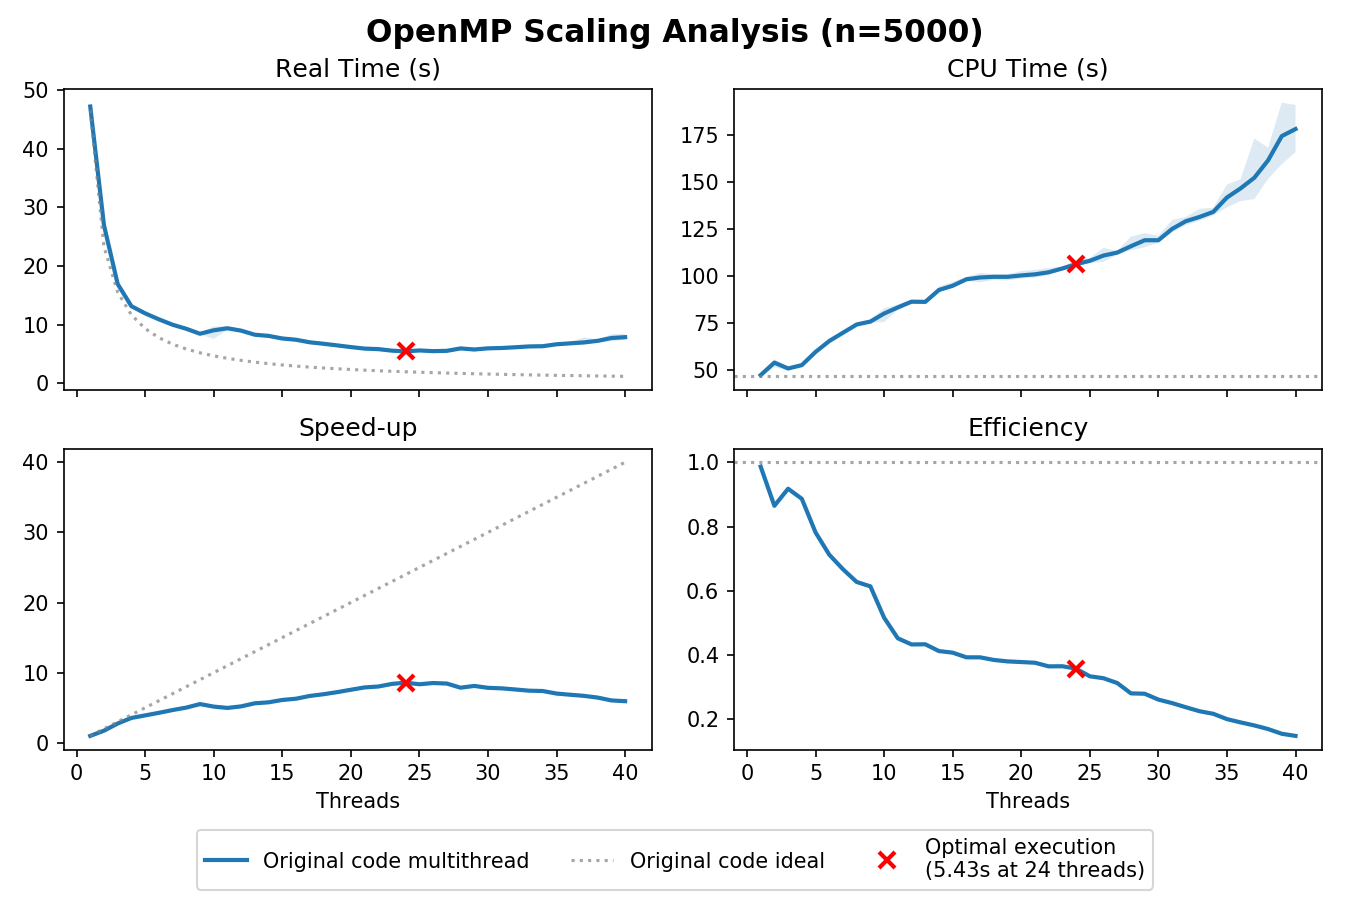
\includegraphics[width=\textwidth]{Images/orig_t_tuning.png}
    \caption{Hyper-parameter tuning of the naive algorithm on $T$, evaluated on matrix \texttt{n=5000} }
    \label{fig:orig_tune_t}
\end{figure}

Comparing these results with the equivalent sequential baseline (which computes a matrix of size \texttt{n=5000} in \textbf{6.5 seconds}), we evaluated the multi-threaded execution using the \emph{Speed-up} and \emph{Efficiency} metrics (introduced in Section~\ref{subsubsec:metrics}). 

The results show a performance degrated so much that it cannot only be caused by multi-threading overhead operations: investigating the compiler's optimization reports clearly shows that introducing the OpenMP directives forces the compiler to avoid the aggressive loop transformations that it typically applies under the \texttt{-O3} flag. 

Once assessed this problem, further hyper-parameter tuning of the naive algorithm is futile. Consequently, we will abandon this implementation and transition to exploring only our custom BLAS-like implementation.





\subsection{BLAS-like implementation}
Given the high complexity of the algorithm (details in Appendix~\ref{subsec:openblas}), it could be modified in several ways (e.g., each thread having its own \texttt{packedA} and \texttt{packedB}, or sharing \texttt{packedB} while keeping \texttt{packedA} private).

Ultimately, the empirically proven best choice is the one proposed in Listing~\ref{lst:blas_like_openmp}: each thread allocates its own \texttt{packedA} and \texttt{packedB} structures and works only on its assigned subset of rows (the \texttt{\#pragma omp for} directive subdivides the workspace of that iteration).

This proved to be the optimal approach because the high capacity of the L3 cache (30 MB) can easily store all the \texttt{packedB} blocks across the threads. Each \texttt{packedB} block is $512 \times 256 \times 8$ bytes (1 MB), meaning the L3 cache can comfortably accommodate up to 30 of them. Additionally, each L2 cache (1.25 MB) can efficiently fit up to two \texttt{packedA} blocks, as each one is $256 \times 256 \times 8$ bytes (0.5 MB).

\begin{lstlisting}[style=CStyle, caption={Blas-like implementation with OpenMP directives}, label={lst:blas_like_openmp}]
extern int n_threads;
extern omp_sched_t runtime_schedule_type;
extern int block_size;

void multiply_matrices( int n, 
    double (*restrict A)[n], 
    double (*restrict B)[n], 
    double (*restrict C)[n]) 
{
    
    (*@\textcolor{red}{omp\_set\_schedule(runtime\_schedule\_type, block\_size);} @*)
    (*@\textcolor{red}{omp\_set\_num\_threads(n\_threads);} @*)    
    
    (*@\textcolor{red}{\#pragma omp parallel shared(A, B, C, n)} @*)   
    {
        const PackedA_t packedA = _mm_malloc(MC * KC * sizeof(double), 64);
        const PackedB_t packedB = _mm_malloc(NC * KC * sizeof(double), 64);

        (*@\textcolor{red}{\#pragma omp for schedule(runtime)} @*)   
        for (int j = 0; j < n; j += NC) {
            int nc = MIN(NC, n - j);
            
            for (int k = 0; k < n; k += KC) {
            
                int kc = MIN(KC, n - k);                
                pack_B(n, B, packedB, k, j, kc, nc);  
                
                for (int i = 0; i < n; i += MC) {
                
                    int mc = MIN(MC, n - i);                    
                    pack_A(n, A, packedA, i, k, mc, kc);
                    
                    for (int ir = 0; ir < mc; ir += MR)
                        for (int jr = 0; jr < nc; jr += NR)
                            kernel_4x8(n, C,
                                    packedA[ir / MR],
                                    packedB[jr / NR],
                                    kc, i + ir, j + jr);
                }
            }
        }

        _mm_free(packedA);
        _mm_free(packedB);
    }
}
\end{lstlisting}

Notably, this approach introduces significant memory bandwidth overhead. Because the \texttt{\#pragma omp for} directive distributes the outer $j$ loop, each thread must independently execute \texttt{pack\_A}, thereby redundantly fetching and packing the exact same blocks of matrix $A$ from main memory $T$ times. Resolving this redundancy is non-trivial; it requires abandoning simple loop-level parallelization in favor of a Single Program, Multiple Data (SPMD) architecture with explicit thread synchronization barriers to safely share packed buffers \footnote{As demonstrated in Section~\ref{subsec:openmp_comparisons}, state-of-the-art (SOTA) libraries substantially outperform this baseline. SOTA implementations, such as OpenBLAS, achieve peak memory bandwidth by dynamically sharing packed buffers across thread teams and utilizing hardware-specific cache-aware optimizations.}. 

Furthermore, we were not capable of acquiring a fully working and readable implementation of those optimizations (to conduct a in-depth analysis). Consequently, this OpenMP integrations is considered sufficient for the purposes of this baseline empirical evaluation.

\subsubsection{Concurrency}
We can now start again with the assessment of the performance of the algorithm as the number of threads changes. Since now the performances are comparable with  the sequential implementation, the matrix size was set to \texttt{n=15000} and every evaluation was repeated for \texttt{3} iterations.

\begin{figure}[H]
    \centering
    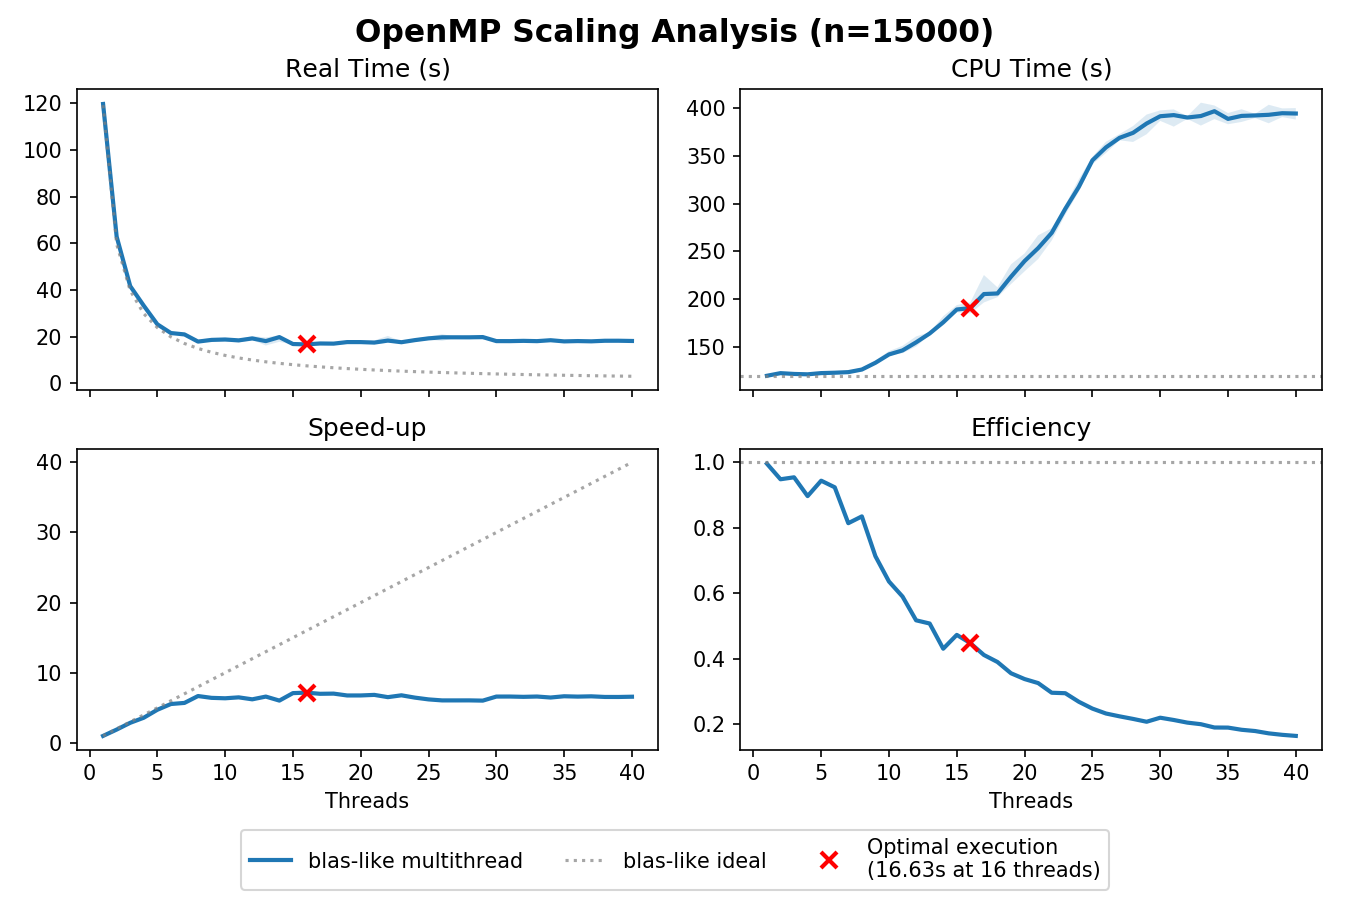
\includegraphics[width=0.85\textwidth]{Images/blas_like_t_tuning.png}
    \caption{Hyper-parameter tuning of the blas-like implementation on $T$, evaluated on matrix \texttt{n=15000} }
    \label{fig:blas_like_tune_t}
\end{figure}

The educated guess is confirmed also in this case, in the Figure~\ref{fig:blas_like_tune_t}; the  performance notably improves with $T \leq 6$ with a quasi-perfect \textbf{speed-up} and \textbf{efficiency}. With more threads, the gain  decreases until the improvements are negligible.

The \textbf{performance degradation} is further motivated by the roofline analysis in Figure~\ref{fig:blas_intel_advisor}: notably, the performance drops from $\approx 59.18 \text{ GFLOPS}$ ($\approx 92\%$ of the \textbf{DP Vector FMA Peak} of $63.71 \text{ GFLOPS}$ --- as shown in the sequential analysis in Figure~\ref{fig:blas_vs_openblas}) to $54\%$ of the roof defined by a multithreaded \textbf{DP Vector FMA Peak} ($744.58 \text{ GFLOPS}$).

\begin{figure}[H]
\centering
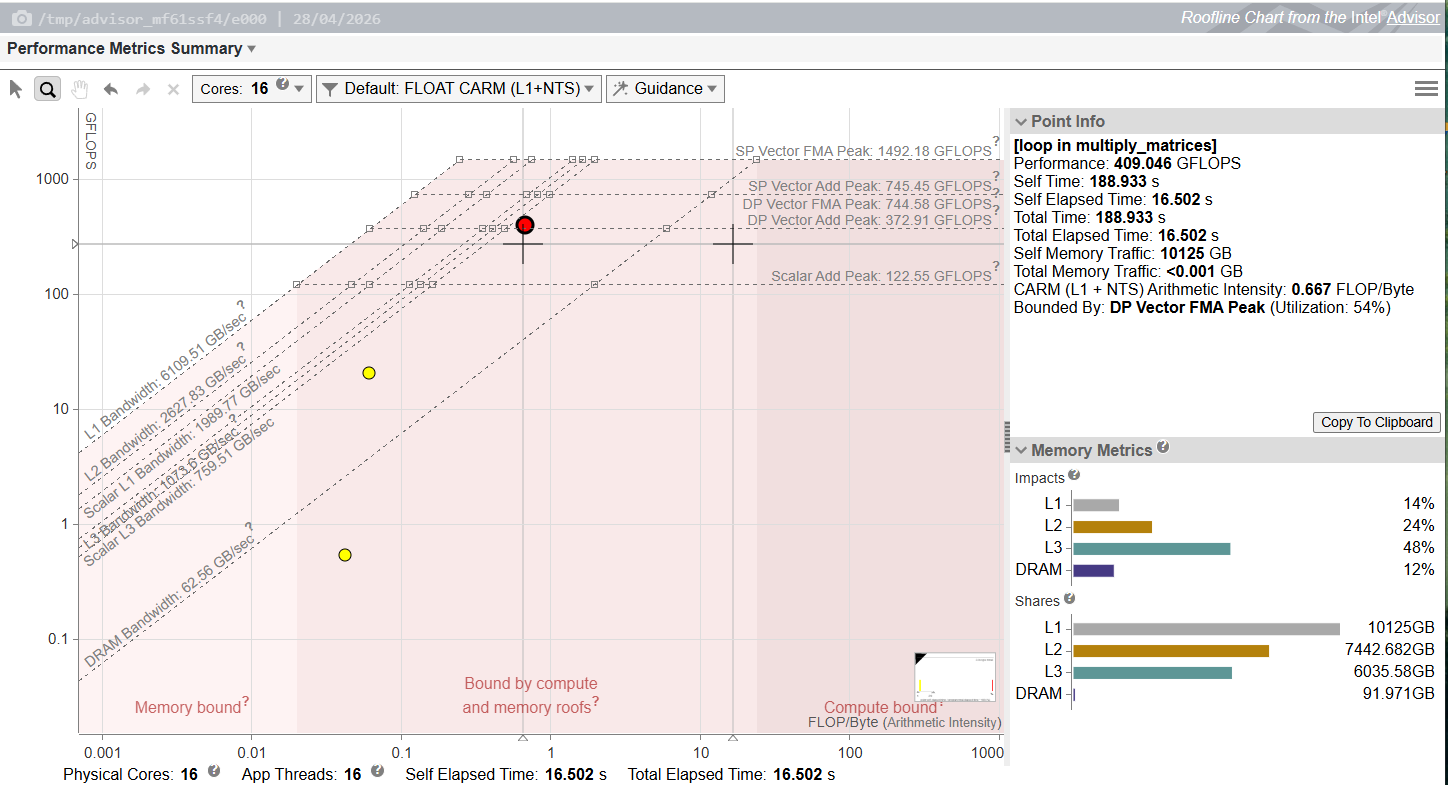
\includegraphics[width=1\textwidth]{Images/blas_intel.png}
\caption{Roofline analysis of our \texttt{Blas-Like} implementatation, executed with \texttt{T=16} on \texttt{n=15000}}
\label{fig:blas_intel_advisor}
\end{figure}

This performance plateau is reflected in the massive data traffic (more than 10,000 GB of L1 traffic, $\approx 48\%$ L3 impact) and low arithmetic intensity. 

\begin{figure}[H]
\centering
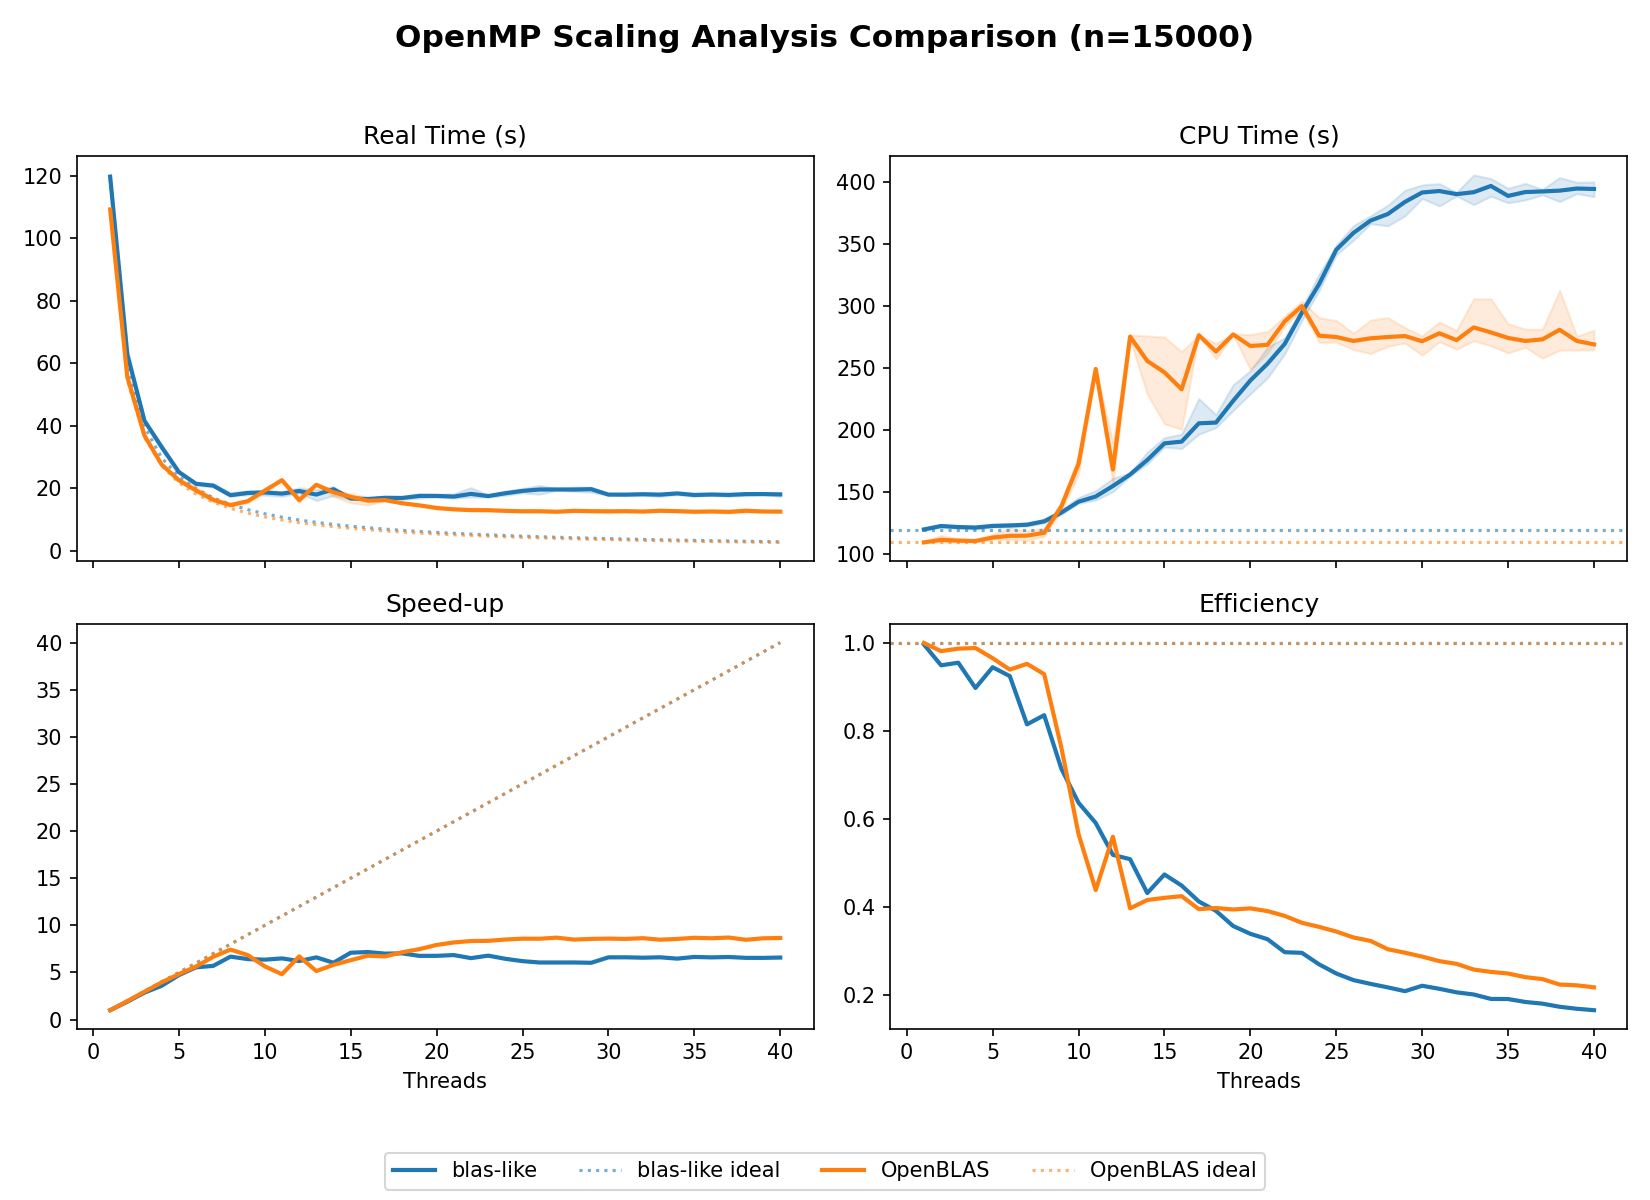
\includegraphics[width=1\textwidth]{Images/blas_comparison_15000.png}
\caption{Performance comparison of the original \texttt{OpenBLAS} and our implementation, in function of \texttt{T} on a matrix \texttt{n=15000}.}
\label{fig:blas_comparison_openmp}
\end{figure}

As Figure~\ref{fig:blas_comparison_openmp} illustrates, even the state-of-the-art OpenBLAS struggles under these constraints; despite a marginally faster absolute execution time, OpenBLAS suffers from severe CPU thrashing beyond 10 threads, yielding a heavily degraded thread efficiency (along with a even more excessive cpu usage).

\vspace{1em}
Having established the inferiority of our implementation, we now attempt to further optimize its multi-thread execution. The pipeline follows a \textbf{greedy approach} to tune the hyperparameters; therefore, for all subsequent tests, the thread count is fixed at \texttt{-{}-threads 16}.

\subsubsection{Scheduling (and Chunk Size)}
To optimize the thread workload, we analyzed the impact of OpenMP scheduling policies (\texttt{static}, \texttt{dynamic}, \texttt{guided}) across varying chunk sizes. Given the matrix size $n=15000$ and a macro-kernel column block $NC=512$, the parallelized outer loop executes  $\lceil 15000 / 512 \rceil = 30$ iterations of the outer (parallelized) loop. 

This coarse granularity, implemented to maximize the usage of the different levels of caches,  dictates the scheduling behavior:
 
\begin{itemize}
    \item \textbf{Thread Starvation (Chunk Size $> 1$):} With only 30 total iterations available to $T=16$ threads, increasing the chunk size immediately causes hardware under-utilization. A chunk size of $2$ yields 15 blocks (leaving 1 thread idle); a chunk size of $8$ leaves 12 threads idle; and any chunk size $\geq 32$ forces purely sequential execution.
    \item \textbf{Load Imbalance:} While the default \texttt{static} policy has minimal overhead, it assumes equal work per iteration. However, the final iteration only computes $15000 \pmod{512} = 152$ columns, finishing significantly faster than the rest. \texttt{static} scheduling forces threads to idle at the implicit barrier while waiting for full-sized chunks to complete.
\end{itemize}

\begin{figure}[H]
    \centering
    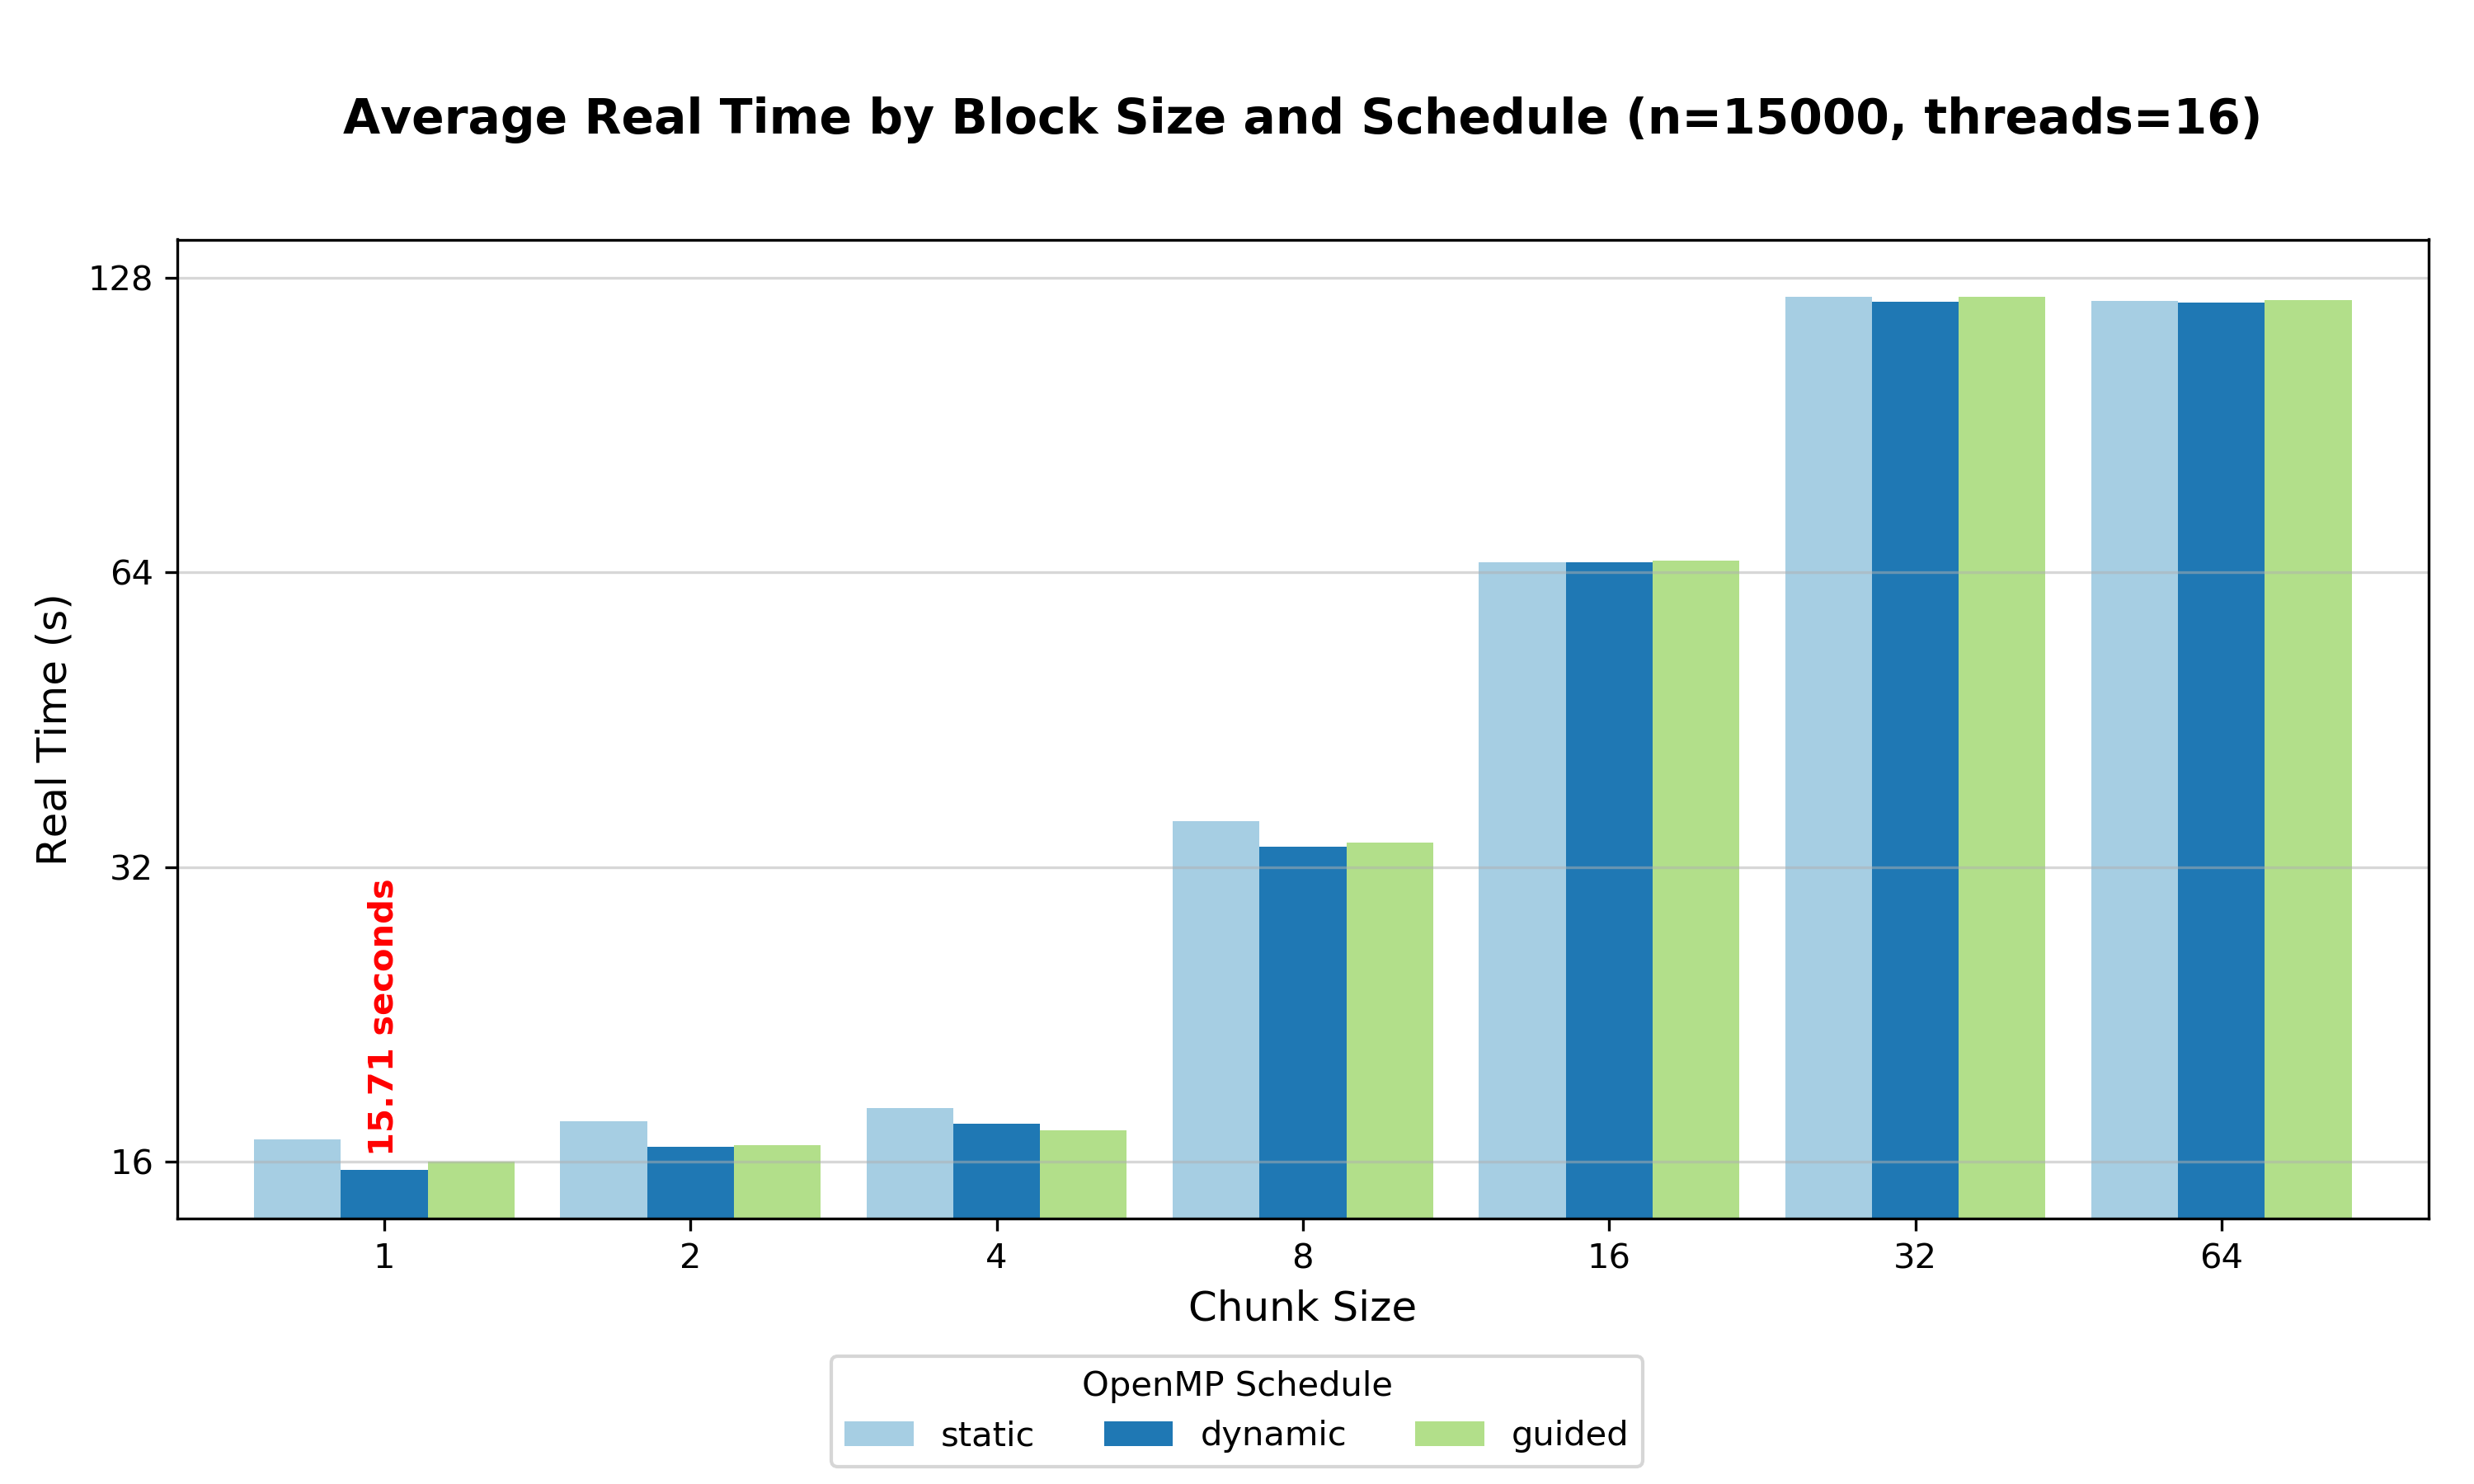
\includegraphics[width=1\textwidth]{Images/blas_like_scheduling.png}
    \caption{Average execution time across varying chunk sizes and scheduling policies, on a matrix n=15000 and T=16.}
    \label{fig:blas_scheduling}
\end{figure}

As demonstrated in Figure~\ref{fig:blas_scheduling}, the margin for improvement is extremely narrow. Configurations with chunk sizes $\geq 8$ result in performance degradation. Consequently, to guarantee full core utilization, the chunk size must be strictly restricted to \texttt{1}. 

Under those observations, the best possible choice is to use the dynamic scheduling by passing   \texttt{-{}-schedule 2 --block-size 1}; this improvement lowers the time down to \textbf{15.71 seconds}.


\subsubsection{Affinity}
Lastly, to (try to) mitigate cache thrashing and maximize hardware utilization, we evaluated the impact of thread affinity. OpenMP controls thread binding through two environment variables:
\begin{itemize}
    \item \texttt{OMP\_PLACES}: Defines the hardware granularity (\texttt{threads}, \texttt{cores}, or \texttt{sockets}) where threads are mapped to be executed.
    \item \texttt{OMP\_PROC\_BIND}: Dictates the distribution policy (\texttt{master}, \texttt{close}, or \texttt{spread}) of threads across the defined places.
\end{itemize}

\begin{figure}[H]
    \centering
    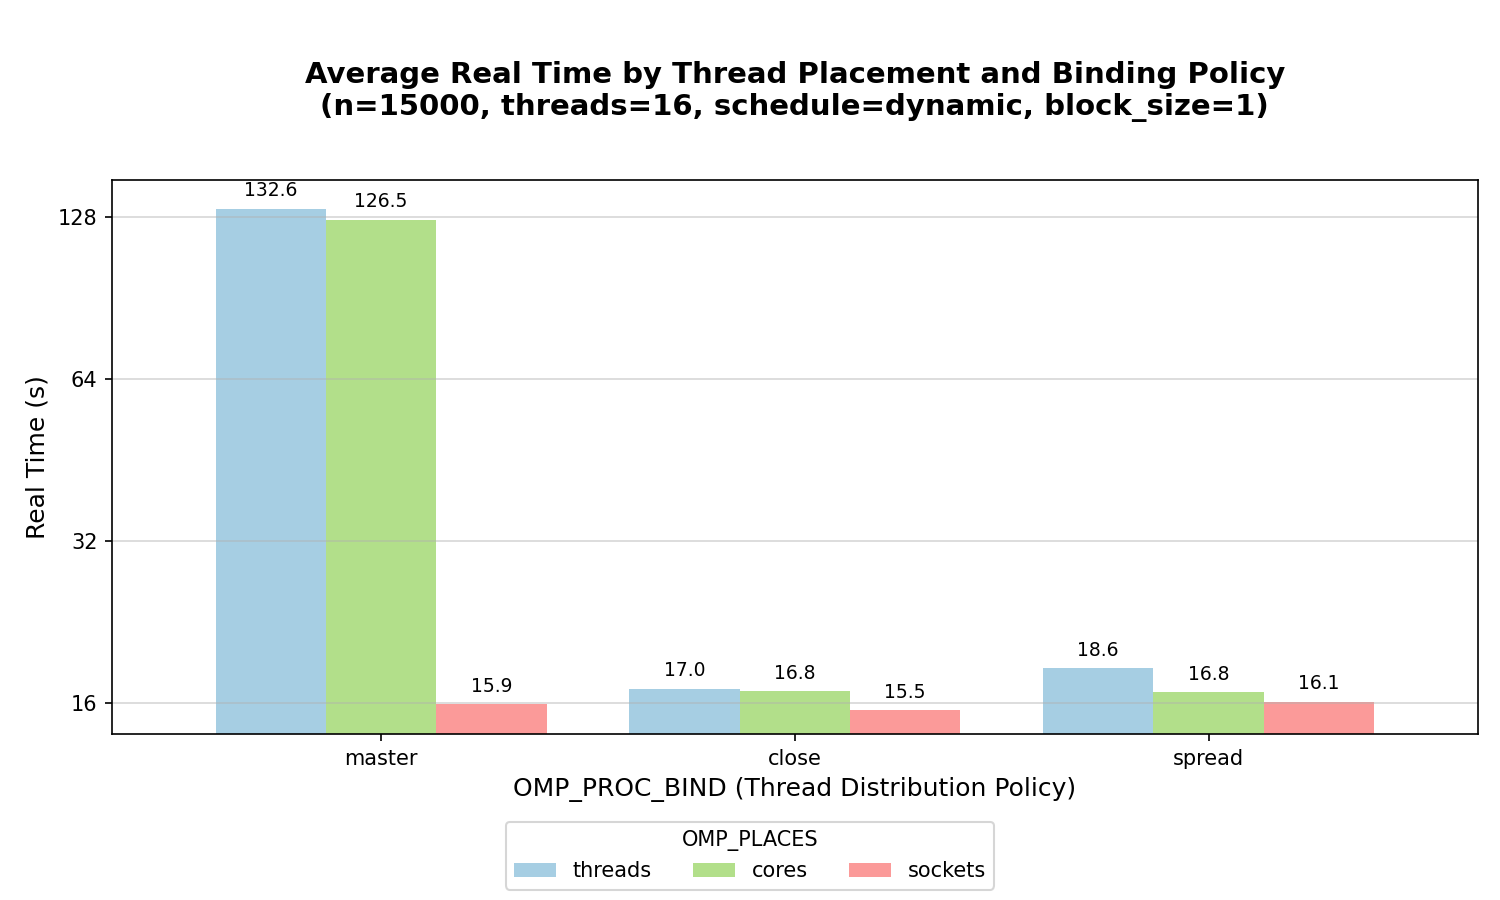
\includegraphics[width=1\textwidth]{Images/blas_like_binding_bind.png}
    \caption{Execution time varying with each possible mapping setting.}
    \label{fig:blas_affinity}
\end{figure}

As illustrated in Figure~\ref{fig:blas_affinity}, the hardware binding configuration can nullify the performance gain of the multithread approach. The \texttt{master} policy catastrophically serializes the workload ($\approx 132\text{s}$) when restricted to a single thread or core, as all 16 threads are forced to multiplex onto a severely limited execution unit. It only recovers when the boundary is expanded to the entire \texttt{socket} (i.e on different cores). 

In contrast, the \texttt{close} and \texttt{spread} policies maintain highly stable performance across all hardware granularities. The absolute optimal configuration is achieved by combining the \texttt{close} policy with \texttt{sockets} ($15.5\text{s}$).



\subsection{Final comparisons}
\label{subsec:openmp_comparisons}

For completeness, we evaluate the performance scaling of the algorithms provided by \texttt{Intel MKL} (Figure~\ref{fig:mkl_tune_t}). Since the library natively manages multithreading, the thread count only needs to be defined dynamically at runtime using its API call \texttt{mkl\_set\_num\_threads(n\_threads)}.

The scaling curves exhibit a clear jagged pattern. This fluctuating behavior is typical of highly optimized libraries like MKL (indeed, it is also present in OpenBLAS, as seen in Figure~\ref{fig:blas_comparison_openmp}). As previously discussed, further speculations regarding these fluctuations is omitted, as they cannot be empirically verified.

\begin{figure}[H]
    \centering
    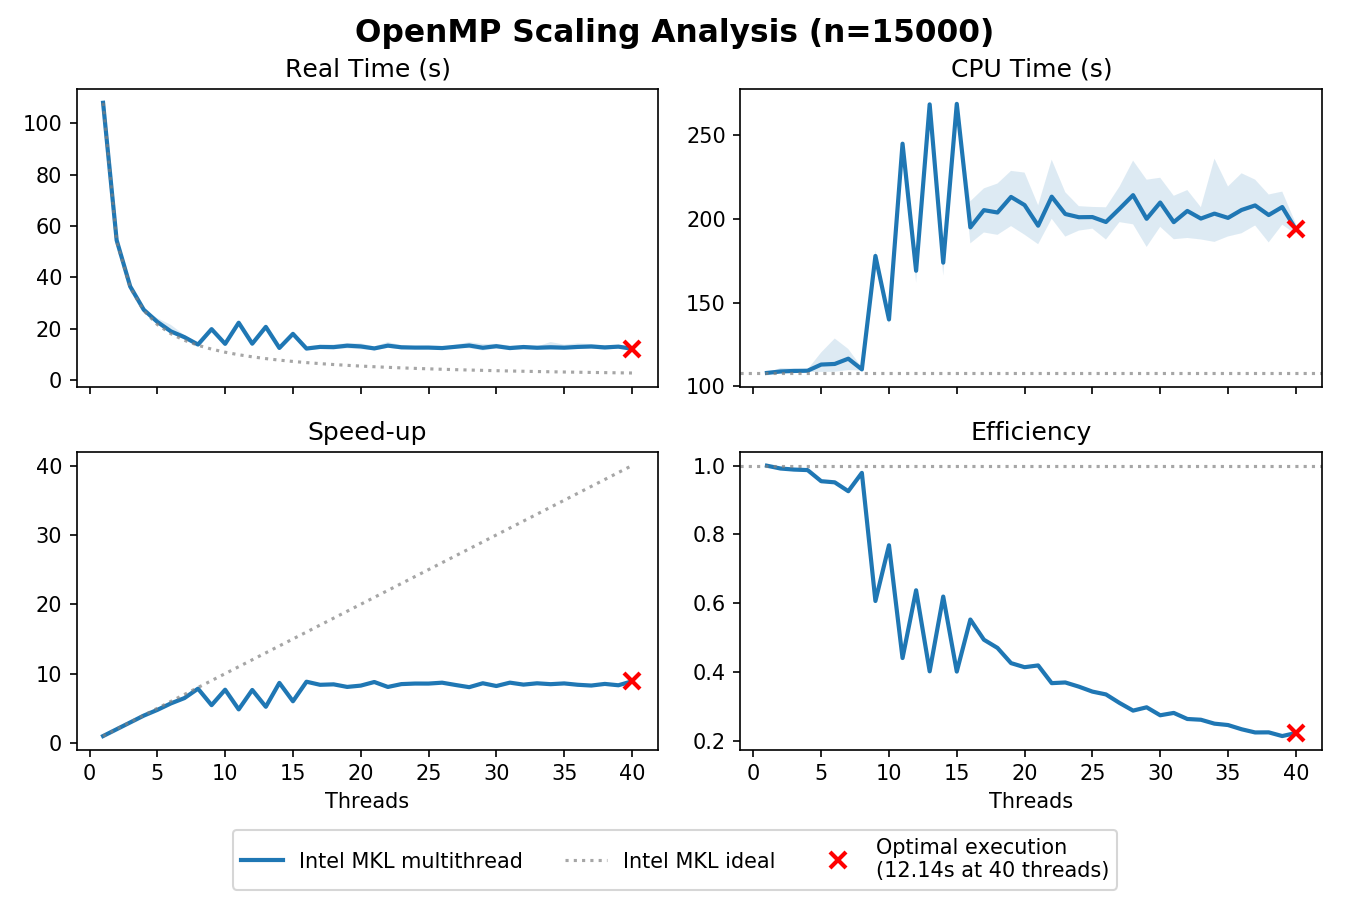
\includegraphics[width=\textwidth]{Images/mkl_t_tuning.png}
    \caption{Hyper-parameter tuning of the Intel MKL implementation on $T$, evaluated on matrix \texttt{n=15000}}
    \label{fig:mkl_tune_t}
\end{figure}


\paragraph{Results Summary}
To summarize the iterative parallel optimization pipeline and contextualize our custom implementations against state-of-the-art libraries, Table~\ref{tab:final_openmp_comparison} aggregates the performance metrics of each major milestone across different matrix sizes.

\begin{table}[H]
\centering
% The resizebox must wrap the ENTIRE threeparttable
\resizebox{\textwidth}{!}{%
  \begin{threeparttable}
    \caption{Performance comparison of the multithreaded implementations across different matrix sizes. Percentages reflect computational throughput (GFLOPS) relative to the Intel MKL baseline. Notably, our version outperform OpenBLAS on bigger matrices.}
    \label{tab:final_openmp_comparison}
    
    \begin{tabular}{l|ccc|ccc|ccc}
    \toprule
     & \multicolumn{3}{c|}{\textbf{N = 5000}} & \multicolumn{3}{c|}{\textbf{N = 10000}} & \multicolumn{3}{c}{\textbf{N = 15000}} \\
    \textbf{Implementation} & \textbf{Time (s)} & \textbf{GFLOPS} & \textbf{\%} & \textbf{Time (s)} & \textbf{GFLOPS} & \textbf{\%} & \textbf{Time (s)} & \textbf{GFLOPS} & \textbf{\%} \\
    \midrule
    Original ($T=24$)                       & 5.360 & 46.65 & 10.01\% & 43.087 & 46.42 & 8.95\% & 149.783 & 45.07 & 8.63\% \\
    Blas-Like ($T=16$, default)             & 0.837 & 298.62 & 64.11\% & 5.789 & 345.47 & 66.62\% & 16.752 & 402.93 & 77.15\% \\
    Blas-Like ($T=16$, dynamic, 1)          & 0.804 & 310.97 & 66.76\% & 4.977 & 401.82 & 77.49\% & 15.571 & 433.49 & 83.00\% \\
    \textbf{Blas-Like (Optimal)}\tnote{1}   & \textbf{0.882} & \textbf{283.32} & \textbf{60.83\%} & \textbf{4.906} & \textbf{407.67} & \textbf{78.61\%} & \textbf{15.571} & \textbf{433.50} & \textbf{83.01\%} \\
    \midrule
    OpenBLAS ($T=16$)                                & 0.662 & 377.37 & 81.02\% & 4.677 & 427.65 & 82.47\% & 16.997 & 397.13 & 76.04\% \\
    \textbf{Intel MKL ($T=16$)}                      & \textbf{0.537} & \textbf{465.77} & \textbf{100.00\%} & \textbf{3.857} & \textbf{518.57} & \textbf{100.00\%} & \textbf{12.925} & \textbf{522.24} & \textbf{100.00\%} \\
    \bottomrule
    \end{tabular}
    
    \begin{tablenotes}
        \footnotesize
        \item[1] Evaluated with tuned affinity settings: \texttt{OMP\_PROC\_BIND=close, OMP\_PLACES=sockets}.
    \end{tablenotes}
  \end{threeparttable}%
}
\end{table}
